\section{Future Work}

Our implementation of the NPRR algorithm has room for many
optimizations. Notable potential optimizations include:

\begin{itemize}
\item The computation of indices on demand, to avoid the creation of
  unused indices
\item The use of constant-width bitmasked vectors to repreest tuples,
  to avoid the expensive copy operations needed for projection
\end{itemize}

However, the most important next step in the development of this
algorithm would be an implementation into an RDBMS such as Postgres.

\subsection{Integration into Postgres}

We conducted extensive study into the feasibility of integrating the
NPRR join into Postgres.

The complexity of adding new types of joins to Postgres has been
greatly reduced by the addition of Custom Scan Providers
[\cite{customscan}] in the development branch of Postgres 9.5. Custom
scan providers allow the insertion of nodes tagged ``custom'' into
Postgres's internal data structures. When encountering one of these
nodes, Postgres will call certain externally-defined functions when it
needs to do things such as render the node or execute a scan. A
Custom Scan Provider provides implementations for these functions,
enabling the addition of new join and scan types simpling by linking
in a dynamic library.

\subsubsection{Lifecycle of a Join}

\begin{figure}[h]
\label{fig:join_lifecycle}
\begin{center}
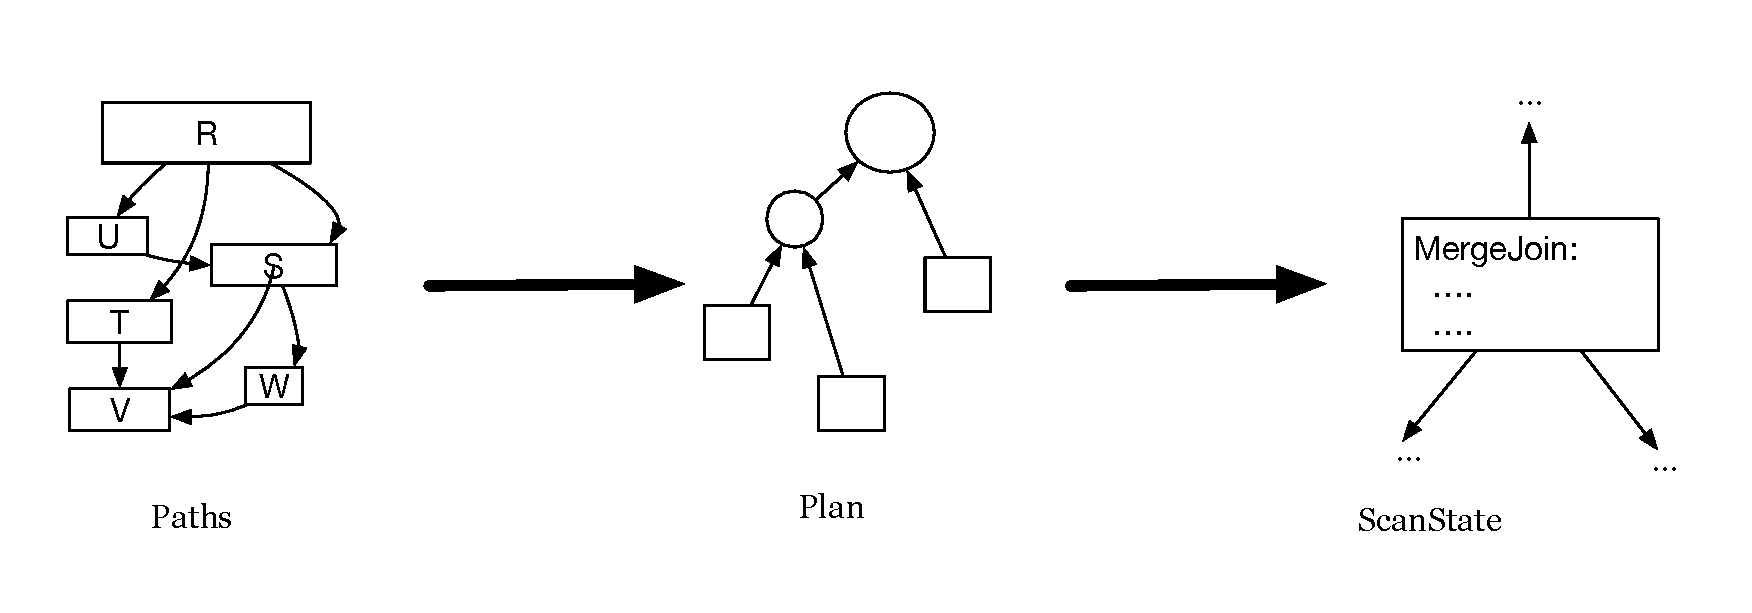
\includegraphics[scale=0.5]{join_lifecycle.pdf}
\end{center}
\caption{Lifecycle of a join in Postgres}
\end{figure}

Whatever the integration mechanism, Implementing a join in Postgres
ultimately requires integrating into the three
subsystems involved in join processing: query planning, plan representation, and query
execution. The query planner constructs a structure of type {\tt
  RelOptInfo} for each relation to be computed during the query, and
then builds a directed acyclic graph of ``paths'' presenting various
ways these relations can be computed from each other. Once the paths
have been considered, an optimal path is selecetd and converted into a
query plan tree. During query execution, every node of the plan tree is
given an associated ``ScanState'' structure. The executor function for
the node is then responsible for computing the next tuple, updating
the scan state and executing the plans for its child nodes. Figure
\ref{fig:join_lifecycle} illustrates the lifecycle of a
join in Postgres. While extending the representation of query plans is
straightforward, the unusual nature of the NPRR join presents problems
for integrating into both the executor and the planner.

\subsubsection{Integrating into the Query Optimizer}

Conventional query planning as implemented in Postgres assumes at most
two children per node, which makes adding the NPRR join difficult. Postgres contains two query planners: the Genetic Query Optimizer
(GEQO), and a standard dynamic-programming based optimizer.

The Genetic Query Optimizer runs a genetic algorithm to iteratively
optimize a pool of potential query plans. Its mechanism for
considering new joins fundamentally only considers pairwise joins. During its process for creating
new individuals, it contains a list of ``clumps,'' or subtrees
together. It is presented with new clumps according to an order suggested by
the genetic algorithm, and considers the cost of joining the new clump pairwise
to any existing clump.

The ``standard join search'' is a Selinger-type DP-based
optimizer. Like other Selinger-type optimizers and similar to the
Genetic Query Optimizer, it maintains optimal subplans for executing
subsets of the query, and iteratively adds new base relations to the
plan by joining individual base relations to an existing subtree with
a pairwise join.

Both optimizers hence do not admit a non-binary join in their search process. We do however have one saving grace that makes the integration of the NPRR
join into the query planner possible, if not feasible. New plans are considered in Postgres using an imperative API. That is,
rather than e.g.: invoking a planning routine which returns a new path
to be considered, each {\tt RelOptInfo} maintains a list of optimal paths
for computing that relation. A planning routine is expected to modify
this list to add new potential joins, possibly pruning strictly
inferior paths. At certain points during query optimization, Postgres
invokes a routine to be implemented by a Custom
Scan Provider. A Custom Scan Provider that offers the NPRR join could
use this to replace all existing paths with one representing an NPRR
join. Properly considering trees that include NPRR joins alongside
traditional pairwise joins would unfortunately require the
implementation of a new search algorithm.

\subsubsection{Integrating into the Query Executor}

The NPRR join requires more substantial preprocessing than other join,
involving the creation of quadratically many hash tables. While Postgres has built-in infrastructure for creating hash indices,
the existing hash index support is hardcoded to only index an entire
table, and to only work on base relations. We would thus need to
implement the indexing ourselves, including handling the buffer
management policies. Joins in Postgres are given great leeway to manage their internal
state, so this issue is less prohibitive than with the query
optimizer. Proper index management would still nonetheless be very difficult.

\subsection{Distributed NPRR in Spark}
We also implemented a basic implementation of NPRR in Spark which computes the join across a distributed cluster of nodes. This raises an interesting question: do the worst-case optimality guarantees of NPRR translate to the distributed setting? Moreover, what does it mean for a join algorithm to be worst-case optimal in the distributed setting? This is a future area of research that could impact large-scale data processing in cluster computing environments and is certainly worth pursuing.